\section{Tests}
Die Tests, die w�hrend der Fachstudie in Nexus-Labor mit der Test-Hardware 
durchgef�hrt wurden, sind in diesen Abschnitt detalliert beschrieben.

\subsection{Hardware}
\begin{itemize}
	\item 2 PCs mit \emph{Wistron CM9 Atheros AR5213A} Wlan Karten
  \item 1 Laptop mit Intel mini-PCI Wlan Karte
\end{itemize}

\subsection{Software}

\subsubsection{Madwifi}

Treiber sind nur fur Fedora 2.6.18 kernel!!!

1. Treiber installieren

\begin{verbatim}
	# svn checkout http://svn.madwifi.org/madwifi/trunk madwifi	
	# cd madwifi	
	# make	
	# make install
\end{verbatim}

2a. Treiber manuell laden 

\begin{verbatim}
	# modprobe ath_pci
\end{verbatim}

2b. Treiber automatisch laden

\begin{verbatim}
	# mkdir /etc/modules.autoload.d/
	# echo ath_pci >> /etc/modules.autoload.d/kernel-2.6
\end{verbatim}

3a. Network-Config automatisch

Datei erstellen:

\begin{verbatim}
	/etc/sysconfig/network-scripts/ifcfg-ath1
\end{verbatim}

und editieren..

\begin{verbatim}
	# Silicon Integrated Systems [SiS] SiS900 PCI Fast Ethernet
	DEVICE=ath1
	ONBOOT=yes
	
	BOOTPROTO=static
	IPADDR=192.168.2.1x
	NETMASK=255.255.255.0
	
	ESSID=mesh
	MODE=ad-hoc
	CHANNEL=36 # 5.18 GHz
	KEY=s:0nexus0suxen0
	# 108-Bit WEP 13 zeichen
\end{verbatim}

3b. Network-Config manuel

\begin{verbatim}
	# iwlist ath1 frequency
	
	          Channel 01 : 2.412 GHz
	          Channel 02 : 2.417 GHz
	          Channel 03 : 2.422 GHz
	          Channel 04 : 2.427 GHz
	          Channel 05 : 2.432 GHz
	          Channel 06 : 2.437 GHz
	          Channel 07 : 2.442 GHz
	          Channel 08 : 2.447 GHz
	          Channel 09 : 2.452 GHz
	          Channel 10 : 2.457 GHz
	          Channel 11 : 2.462 GHz
	          Channel 36 : 5.18 GHz
	          Channel 40 : 5.2 GHz
	          Channel 42 : 5.21 GHz
	          Channel 44 : 5.22 GHz
	          Channel 48 : 5.24 GHz
	          Channel 50 : 5.25 GHz
	          Channel 52 : 5.26 GHz
	          Channel 56 : 5.28 GHz
	          Channel 58 : 5.29 GHz
	          Channel 60 : 5.3 GHz
	          Channel 64 : 5.32 GHz
	          Channel 149 : 5.745 GHz
	          Channel 152 : 5.76 GHz
	          Channel 153 : 5.765 GHz
	          Channel 157 : 5.785 GHz
	          Channel 160 : 5.8 GHz
	          Channel 161 : 5.805 GHz
	          Channel 165 : 5.825 GHz
	          Current Channel=0	
	# ifconfig ath1 inet 192.168.0.1/24	
	# iwconfig ath1 essid mesh
	# iwconfig ath1 mode ad-hoc
	# iwconfig ath1 channel 36
	# iwconfig ath1 enc n1e2x3u4s5
\end{verbatim}


\subsubsection{OLSR Daemon}

1. olsrd installieren 

\begin{verbatim}
	# cvs -d:pserver:anonymous@olsrd.cvs.sourceforge.net:/cvsroot/olsrd login
	# cvs -z3 -d:pserver:anonymous@olsrd.cvs.sourceforge.net:/cvsroot/olsrd co olsrd-current
	# cd olsrd-current
	# make
	# make install
\end{verbatim}

2. Plug-ins fur olsrd installieren 

\begin{verbatim}
# cd lib/"plugin-name"
# make 
# make install 
# chcon -t textrel_shlib_t /usr/lib/olsrd_httpinfo.so.0.1 (!)
\end{verbatim}

3. olsrd kofigurieren

\begin{itemize}
	\item Datei /etc/olsrd.conf erstellen und editieren!!! (sieh file) 
	\item TCP Port 8080 fur Httpinfo und 8081 fur Dot UDP 698 fur Eingehende 
				Pakete erlauben. Datei /etc/sysconfig/iptables editieren: 
\end{itemize}

\begin{verbatim}
-A RH-Firewall-1-INPUT -p tcp --dport 8080 -m state --state NEW -j ACCEPT
-A RH-Firewall-1-INPUT -p tcp --dport 8081 -m state --state NEW -j ACCEPT
-A RH-Firewall-1-INPUT -i ath1 -p udp --sport 698 -j ACCEPT
\end{verbatim}

4. olsrd starten 

\begin{verbatim}
 # olsrd
\end{verbatim}


\subsection{Topologie}
\wlanimage{Topology}{Topologie}

\subsection{Ergebnisse}
%\wlanimage{Olsr_Route}{Http Info}
    \begin{figure}[H]
      \centering
      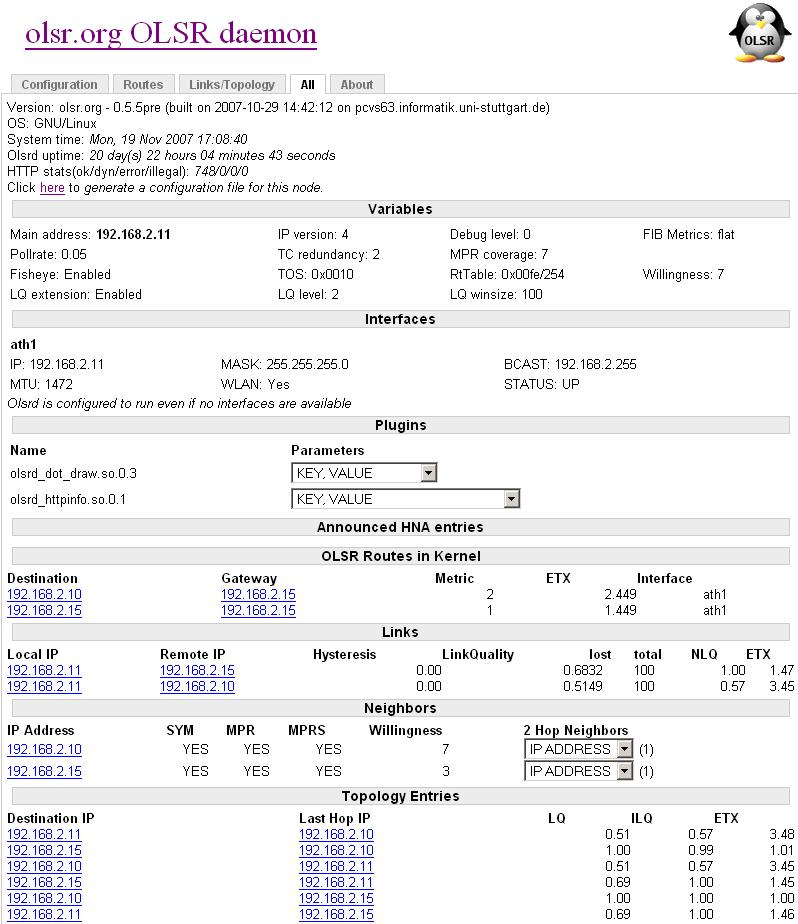
\includegraphics[width=1.0\textwidth]{images/Olsr_Route.jpg}
      \caption{Http Info}
      \label{fig:Olsr_Route}
    \end{figure}